\documentclass[a4paper,12pt]{article}
\usepackage{graphicx}
\usepackage{caption}
\usepackage{subcaption}
\usepackage{float}
\usepackage[margin=1in]{geometry}
\usepackage{lmodern}
\usepackage{amsmath}
\usepackage{xcolor}
\usepackage{listings}
\usepackage{pgffor}

\lstset{
  breaklines=true,
  postbreak=\mbox{\textcolor{red}{$\hookrightarrow$}\space},
}

\graphicspath{{../../python/kNN/k_optimization/results/}}

\begin{document}

\title{Relatório kNN}
\author{Eduardo}
\date{\today}
\maketitle

\section*{Exercício 1}

As figuras a seguir apresentam a relação entre número de vizinhos, \texttt{k}, e a precisão média na validação /textit{k-fold} para três dados reais.

\begin{figure}[H]
  \centering
  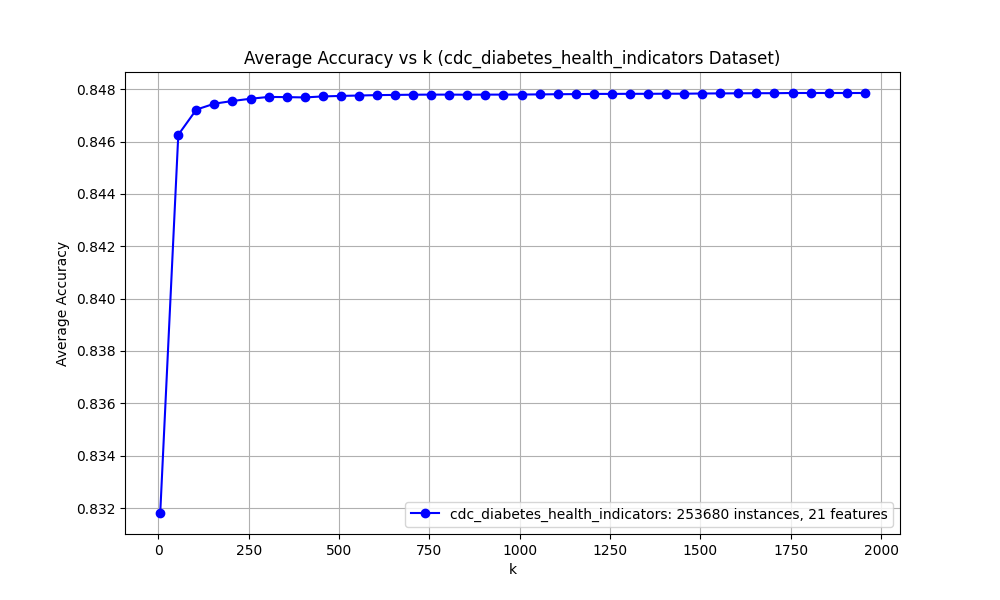
\includegraphics[width=0.6\textwidth]{cdc_diabetes_health_indicators.png}
  \caption{Relação entre número de vizinhos (\texttt{k}) e precisão média para o conjunto de dados \texttt{cdc\_diabetes\_health\_indicators}.}
  \label{fig:cdc_diabetes_health_indicators}
\end{figure}

\begin{figure}[H]
  \centering
  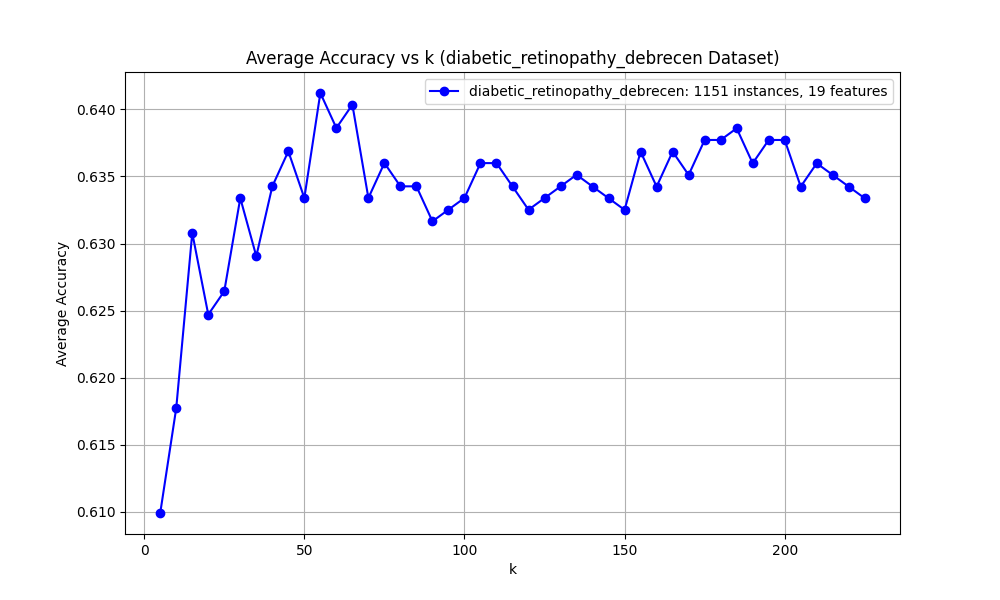
\includegraphics[width=0.6\textwidth]{diabetic_retinopathy_debrecen.png}
  \caption{Relação entre número de vizinhos (\texttt{k}) e precisão média para o conjunto de dados \texttt{diabetic\_retinopathy\_debrecen}.}
  \label{fig:diabetic_retinopathy_debrecen}
\end{figure}

\begin{figure}[H]
  \centering
  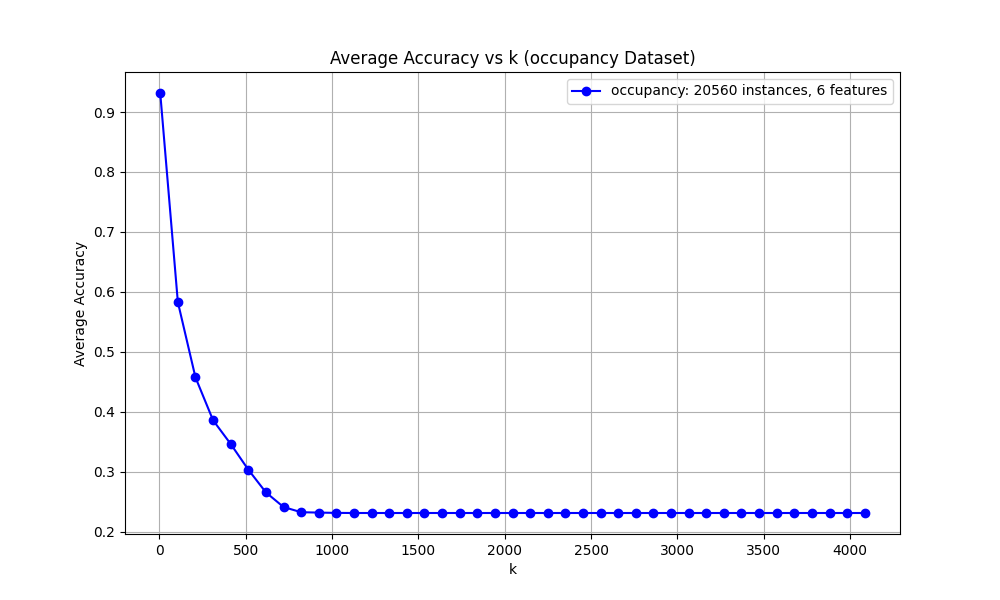
\includegraphics[width=0.6\textwidth]{occupancy.png}
  \caption{Relação entre número de vizinhos (\texttt{k}) e precisão média para o conjunto de dados \texttt{occupancy}.}
  \label{fig:occupancy}
\end{figure}

Nota-se que o número ótimo de vizinhos muda conforme o conjunto de dados. Para o encontrar, uma forma eficiente e automática é a aplicação de um otimizador que busque \texttt{k} que maximize a precisão média.

\end{document}
